\documentclass[14pt]{beamer}

\usetheme{Montpellier}
\usecolortheme{beaver}

\usepackage{amsmath, amssymb, ../../vimacros, hyperref, tikz}
\usepackage{../../pdfpcnotes}
\usetikzlibrary{positioning, fit, bayesnet}
\usepackage[round]{natbib}
\usepackage{physics}
\usepackage{verbatim}

\hypersetup{breaklinks=true, colorlinks=true, linkcolor=blue, urlcolor=blue, citecolor=blue}

\beamertemplatenavigationsymbolsempty

\title{Deep Generative Models: \\
Continuous Latent Variables}
\author{Philip Schulz and Wilker Aziz\\
\url{https://github.com/philschulz/VITutorial}}
\date{}

\setbeamertemplate{footline}[frame number]

\begin{document}

\begin{frame}
\maketitle
\end{frame}

\frame{\tableofcontents}

\section{Deep Generative Models}
\frame{\tableofcontents[currentsection]}

\begin{frame}{Generative Models}
Joint distribution over observed data $ x $ and latent variables $ Z $.
\begin{equation*}
p(x,z|\theta) =  \underbrace{p(z)}_{\text{prior}} \underbrace{p(x|z,\theta)}_{\text{likelihood}}
\end{equation*} 
The likelihood and prior are often standard distributions (Gaussian, Bernoulli) with simple dependence on conditioning
information.
\end{frame}

\begin{frame}{Deep generative models}

Joint distribution with {\bf deep observation model}
\begin{equation*}
p(x, z|\theta) = \underbrace{p(z)}_{\text{prior}} \underbrace{p(x|z, \theta)}_{\text{likelihood}}
\end{equation*}
~ {\small mapping from $z$ to $p(x|z, \theta)$ is a NN with parameters $\theta$}

~ \pause

Marginal likelihood 
\begin{equation*}
p(x|\theta) = \int p(x, z|\theta) \dd{z} = \int p(z)p(x|z, \theta) \dd{z} 
\end{equation*}
~ \alert{intractable} in general



\end{frame}


\begin{frame}{Goals}

\pnote{Q: Why is gradient-based MLE not possible?}

We want
\begin{itemize}
	\item richer probabilistic models  \pause
	\item complex observation models \\
	parameterised by NNs 
	%\item but we cannot use backprop for parameter estimation \\
	%due to intractability of log-marginal and its gradient
\end{itemize}
\pause
but we can't perform gradient-based MLE

~

\pause

We need \alert{approximate inference} techniques!

\end{frame}

\begin{comment}  % TODO: move this closer to VAE
\begin{frame}{Recap: Variational Inference}
\begin{block}{Objective}
\begin{equation*}
\underset{q(z)}{\max}~\E{\log p(x,z)} + \Ent{q(z)}
\end{equation*}
\begin{itemize}
\item The ELBO is a lower bound on $ \log p(x) $
\item Mean field assumption: $ q(z) = \prod_{i=1}^{N}q(z_{i}) $
\end{itemize}
\end{block}
\end{frame}
\end{comment}


\section{First Attempt: Wake-Sleep}
\frame{\tableofcontents[currentsection]}

\begin{frame}{Wake-sleep Algorithm}
\begin{itemize}
\item Generalise latent variables to Neural Networks
\item Train generative neural model
\item Use variational inference! (kind of)
\end{itemize}
\end{frame}

\begin{frame}{Wake-sleep Architecture}
2 Neural Networks:
\begin{itemize}
\pause
\item A generation network to model the data (the one we want to optimise) -- parameters: $ \theta $
\pause
\item An inference (recognition) network (to model the latent variable) -- parameters: $ \lambda $
\pause
\item Original setting: binary hidden units
\pause
\item Training is performed in a ``hard EM'' fashion
\end{itemize}
\end{frame}

\begin{frame}{Wake-sleep Training}
\textbf{Wake Phase} \\
\begin{itemize}
\item Use inference network to sample hidden unit setting $ z $ from $ q(z|x,\lambda) $
\item Update generation parameters $ \theta $ to maximize join log-liklelihood of data and latents $ p(x,z|\theta) $
\end{itemize}
\pause
\textbf{Sleep Phase}
\begin{itemize}
\item Produce dream sample $ \tilde{x} $ from random hidden unit $ z $
\item Update inference parameters $ \lambda $ to maximize probability of latent state $ q(z|\tilde{x},\lambda) $
\end{itemize}
\end{frame}

\begin{frame}{Wake Phase Objective}
Objective  %

\vspace{-15pt}

\begin{equation*}
\begin{aligned}
&\min_{\theta} \KL{q(z|x, \lambda)}{p(z|x, \theta)} \\ \pause
&= \max_{\theta}~ \underbrace{\mathbb E_{q(z|x, \lambda)}\left[ \log p(z, x| \theta) \right] + \mathbb H[q(z|x, \lambda)]}_{\mathcal G(\theta)}  \pause
\end{aligned}
\end{equation*}

Gradient estimate

\begin{equation*}
\begin{aligned}
\grad_\theta \mathcal G(\theta) &= \mathbb E_{q(z|x, \lambda)}\left[ \grad_\theta \log p(z, x| \theta) \right] + \grad_\theta \mathbb H[q(z|x, \lambda)] \\ \pause
&\overset{\text{MC}}{\approx} \grad_\theta \log p(z, x| \theta) 
\end{aligned}
\end{equation*} 
~ with $ z $ drawn from $ q(z|x,\lambda) $ 
\end{frame}

\begin{frame}{Wake Phase Objective}

Assumes latent state $ z $ to be fixed random draws from $ q(z|x,\lambda) $.

\begin{equation*}
\begin{aligned}
&\min_{\theta} \KL{q(z|x, \lambda)}{p(z|x, \theta)} \\ 
&\overset{\text{MC}}{\approx} \max_\theta \log p(z, x| \theta) 
\end{aligned}
\end{equation*} 

This is simply supervised learning with imputed latent data!

\end{frame}


\begin{frame}{Wake Phase Sampling}
\begin{figure}
\center
\begin{tikzpicture}
\node[draw, circle] (z3) {$ z_{3} $};

\node[draw, circle, below left =of z3] (z1) {$ z_{1} $};
\node[draw, circle, below right = of z3] (z2) {$ z_{2} $};

\node[draw, rectangle,  below left= of z1] (in1) {$ x_{1} $};
\node[draw, rectangle, below left=of z2] (in2) {$ x_{2} $}; 
\node[draw, rectangle, below right= of z2] (in3) {$ x_{3} $};
\end{tikzpicture}
\end{figure}
\end{frame}

\begin{frame}{Wake Phase Sampling}
\begin{figure}
\center
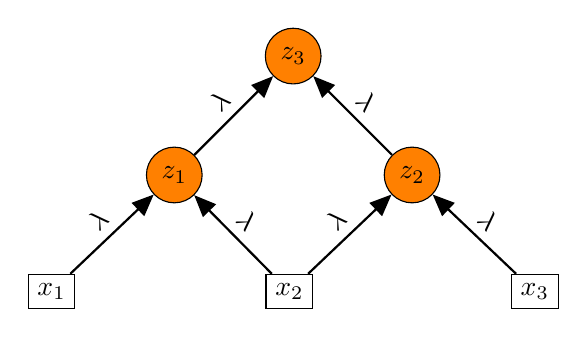
\begin{tikzpicture}
\node[draw, circle, fill=orange] (z3) {$ z_{3} $};

\node[draw, circle, fill=orange, below left =of z3] (z1) {$ z_{1} $};
\node[draw, circle, fill=orange, below right = of z3] (z2) {$ z_{2} $};

\node[draw, rectangle,  below left= of z1] (in1) {$ x_{1} $};
\node[draw, rectangle, below left=of z2] (in2) {$ x_{2} $}; 
\node[draw, rectangle, below right= of z2] (in3) {$ x_{3} $};

\draw[->, thick] (in1) -- (z1) node[midway, above, rotate=45] {$ \lambda $};
\draw[->, thick] (in2) -- (z1) node[midway, above, rotate=315] {$ \lambda $};
\draw[->, thick] (in2) -- (z2) node[midway, above, rotate=45] {$ \lambda $};
\draw[->, thick] (in3) -- (z2) node[midway, above, rotate=315] {$ \lambda $};
\draw[->, thick] (z1) -- (z3) node[midway, above, rotate=45] {$ \lambda $};
\draw[->, thick] (z2) -- (z3) node[midway, above, rotate=315] {$ \lambda $};
\end{tikzpicture}
\end{figure}
\end{frame}

\begin{frame}{Wake Phase Update}
\begin{figure}
\center
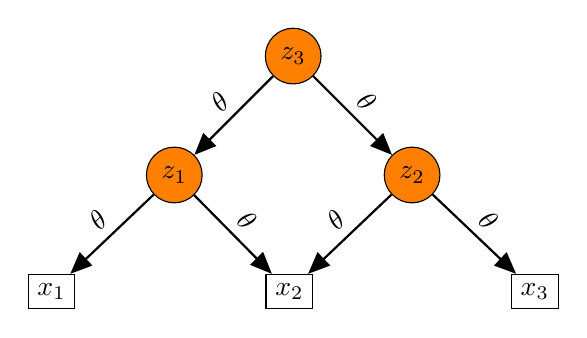
\begin{tikzpicture}
\node[draw, circle, fill=orange] (z3) {$ z_{3} $};

\node[draw, circle, fill=orange, below left =of z3] (z1) {$ z_{1} $};
\node[draw, circle, fill=orange, below right = of z3] (z2) {$ z_{2} $};

\node[draw, rectangle,  below left= of z1] (in1) {$ x_{1} $};
\node[draw, rectangle, below left=of z2] (in2) {$ x_{2} $}; 
\node[draw, rectangle, below right= of z2] (in3) {$ x_{3} $};

\draw[->, thick] (z1) -- (in1) node[midway, above, rotate=45] {$ \theta $};
\draw[->, thick] (z1) -- (in2) node[midway, above, rotate=315] {$ \theta $};
\draw[->, thick] (z2) -- (in2) node[midway, above, rotate=45] {$ \theta $};
\draw[->, thick] (z2) -- (in3) node[midway, above, rotate=315] {$ \theta $};
\draw[->, thick] (z3) -- (z1) node[midway, above, rotate=45] {$ \theta $};
\draw[->, thick] (z3) -- (z2) node[midway, above, rotate=315] {$ \theta $};
\end{tikzpicture}
\end{figure}
\end{frame}


\begin{frame}{Sleep Phase Objective}
Objective  %

\vspace{-15pt}

\begin{equation*}
\begin{aligned}
&\min_{\lambda} \KL{q(z|x, \lambda)}{p(z|x, \theta)} \\ \pause
&= \max_{\lambda}~ \underbrace{\mathbb E_{q(z|x, \lambda)}\left[ \log p(z, x| \theta) \right] + \mathbb H[q(z|x, \lambda)]}_{\mathcal R(\lambda)}  \pause
\end{aligned}
\end{equation*}

Gradient estimate

\vspace{-10pt}
\begin{equation*}
\begin{aligned}
\grad_\lambda \mathcal R(\lambda) &=  \alert{\grad_\lambda} \mathbb E_{q(z|x, \alert{\lambda})}\left[ \log p(z, x| \theta) \right] + \alert{\grad_\lambda} \alert{\mathbb H[q(z|x, \lambda)]} 
\end{aligned}
\end{equation*} 

\pause

\alert{Let's change the objective!}

\end{frame}


\begin{frame}{Sleep Phase Objective}


Assumes fake data $ \tilde{x} $ and latent variables $ z $ to be fixed random draw from $ p(x,z|\theta) $.
\begin{equation*}
\begin{aligned}
&\max_{\lambda}~  \E[p(\tilde x, z|\theta)]{\log q(z|\tilde x, \lambda)} + \mathbb E_{p(\tilde x)}\left[\Ent{p(z|\tilde{x},\theta)}\right] \pause \\
&\overset{\text{MC}}{\approx} \max_{\lambda}~ \log q(z|\tilde x, \lambda)
\end{aligned}
\end{equation*} 

\end{frame}

\begin{frame}{Sleep Phase Sampling}
\begin{figure}
\center
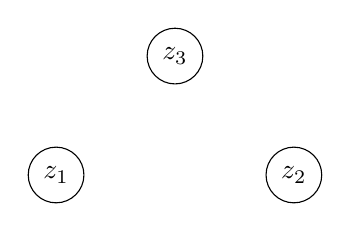
\begin{tikzpicture}
\node[draw, circle] (z3) {$ z_{3} $};

\node[draw, circle, below left =of z3] (z1) {$ z_{1} $};
\node[draw, circle, below right = of z3] (z2) {$ z_{2} $};
\end{tikzpicture}
\end{figure}
\end{frame}

\begin{frame}{Sleep Phase Sampling}
\begin{figure}
\center
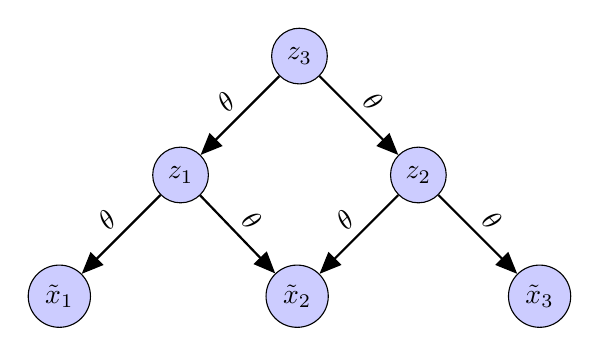
\begin{tikzpicture}
\node[draw, circle, fill=blue!20] (z3) {$ z_{3} $};

\node[draw, circle, fill=blue!20, below left =of z3] (z1) {$ z_{1} $};
\node[draw, circle, fill=blue!20, below right = of z3] (z2) {$ z_{2} $};

\node[draw, circle, fill=blue!20, below left= of z1] (in1) {$ \tilde{x}_{1} $};
\node[draw, circle, fill=blue!20, below left=of z2] (in2) {$ \tilde{x}_{2} $}; 
\node[draw, circle, fill=blue!20, below right= of z2] (in3) {$ \tilde{x}_{3} $};

\draw[->, thick] (z1) -- (in1) node[midway, above, rotate=45] {$ \theta $};
\draw[->, thick] (z1) -- (in2) node[midway, above, rotate=315] {$ \theta $};
\draw[->, thick] (z2) -- (in2) node[midway, above, rotate=45] {$ \theta $};
\draw[->, thick] (z2) -- (in3) node[midway, above, rotate=315] {$ \theta $};
\draw[->, thick] (z3) -- (z1) node[midway, above, rotate=45] {$ \theta $};
\draw[->, thick] (z3) -- (z2) node[midway, above, rotate=315] {$ \theta $};
\end{tikzpicture}
\end{figure}
\end{frame}

\begin{frame}{Sleep Phase Update}
\begin{figure}
\center
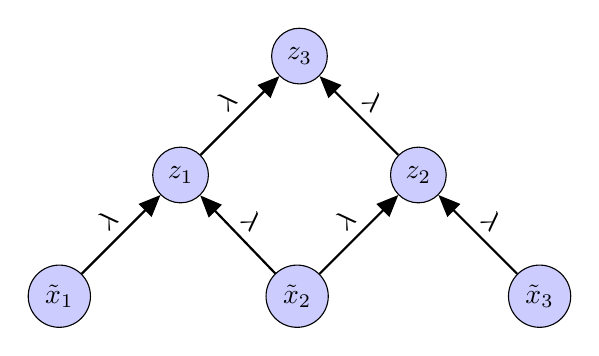
\begin{tikzpicture}
\node[draw, circle, fill=blue!20] (z3) {$ z_{3} $};

\node[draw, circle, fill=blue!20, below left =of z3] (z1) {$ z_{1} $};
\node[draw, circle, fill=blue!20, below right = of z3] (z2) {$ z_{2} $};

\node[draw, circle, fill=blue!20, below left= of z1] (in1) {$ \tilde{x}_{1} $};
\node[draw, circle, fill=blue!20, below left=of z2] (in2) {$ \tilde{x}_{2} $}; 
\node[draw, circle, fill=blue!20, below right= of z2] (in3) {$ \tilde{x}_{3} $};

\draw[->, thick] (in1) -- (z1) node[midway, above, rotate=45] {$ \lambda $};
\draw[->, thick] (in2) -- (z1) node[midway, above, rotate=315] {$ \lambda $};
\draw[->, thick] (in2) -- (z2) node[midway, above, rotate=45] {$ \lambda $};
\draw[->, thick] (in3) -- (z2) node[midway, above, rotate=315] {$ \lambda $};
\draw[->, thick] (z1) -- (z3) node[midway, above, rotate=45] {$ \lambda $};
\draw[->, thick] (z2) -- (z3) node[midway, above, rotate=315] {$ \lambda $};
\end{tikzpicture}
\end{figure}
\end{frame}

\begin{frame}{Wake-sleep Algorithm}
\textbf{Advantages}
\begin{itemize}
\item Simple layer-wise updates
\item Amortised inference: all latent variables are inferred from the same weights $ \lambda $
\end{itemize}
\pause
\textbf{Drawbacks}
\begin{itemize}
\item Inference and generative networks are trained on different objectives
\item Inference weights $ \lambda $ are updated on fake data $ \tilde{x} $
\item Generative weights are bad initially, giving wrong signal to the updates of $ \lambda $
\end{itemize}
\end{frame}

\section{This is how we do: Variational Autoencoders}
\frame{\tableofcontents[currentsection]}

\begin{frame}{Generative Model with NN Likelihood}
\begin{block}{Goal}
Define model $ p(x,z|\theta) = p(x|z,\theta)p(z) $ where the likelihood $ p(x|z,\theta) $ is given by a neural
network. (We fix $ p(z) $ for simplicity.)
\end{block}
\pause
\begin{block}{Problem}
$ p(x) = \intl{p(x|z,\theta) p(z)}{z} $ is hard to compute.
\end{block}
\end{frame}

\begin{frame}{Generative Model with NN Likelihood}
\begin{block}{Goal}
Define model $ p(x,z|\theta) = p(x|z,\theta)p(z) $ where the likelihood $ p(x|z,\theta) $ is given by a neural
network. (We fix $ p(z) $ for simplicity.)
\end{block}
\begin{block}{Problem}
$ p(x) = \intl{\alert{\underbrace{p(x|z,\theta)}_{\substack{\text{highly} \\  \text{non-linear!}}}} p(z)}{z} $ is hard to compute.
\end{block}
\end{frame}

\begin{frame}{Solution: Variational Inference}

\vspace{-10pt}
\begin{small}
\begin{equation*}
\begin{aligned}
\log p(x|\theta) &\geq \overbrace{\E[q(z|x, \lambda)]{\log p(x,Z|\theta)} + \Ent{q(z|x, \lambda)}}^{\ELBO} \\ 
\pause
&= \E[q(z|x, \lambda)]{\log p(x|Z, \theta) + \log p(Z)} + \Ent{q(z|x, \lambda)} \\ \pause
&= \E[q(z|x, \lambda)]{\log p(x|Z, \theta)} - \KL{q(z|x, \lambda)}{p(z)}
\end{aligned}
\end{equation*}
\end{small}

\pause

\vspace{-20pt}
\begin{equation*}
\argmax_{\theta,\lambda} ~ \E[q(z|x, \lambda)]{\log p(x|Z, \theta)} - \KL{q(z|x, \lambda)}{p(z)}
\end{equation*}


\pause

\begin{itemize}
	\item assume $\KL{q(z|x, \lambda)}{p(z)}$  analytical\\
	true for exponential families \pause
	\item approximate $\E[q(z|x, \lambda)]{\log p(x|z, \theta)}$ by sampling\\
	feasible because  $q(z|x, \lambda)$ is simple
\end{itemize}


\end{frame}

\begin{frame}{Generator Network Gradient}
\vspace{-10pt}
\begin{equation*}
\begin{aligned}
&\pdv{\theta}\E[q(z|x,\lambda)]{\log p(x|z,\theta)} - \overbrace{\KL{q(z|x,\lambda)}{p(z)}}^{constant} \\ \pause 
&=\E[q(z|x,\lambda)]{\pdv{\theta}\log p(x|z,\theta)} \\ \pause
&\overset{\text{MC}}{\approx} \frac{1}{S}\sum_{i=1}^{S}
\pdv{\theta} \log p(x|z_{i},\theta) \\
&\textcolor{gray}{\text{where }z_i \sim q(z|x, \lambda)}
\end{aligned}
\end{equation*}
\pause
\center{Note: $ q(z|x,\lambda) $ does not depend on $ \theta $.}
\end{frame}

\begin{frame}{Inference Network Gradient}
\begin{equation*}
\begin{aligned}
&\pdv{\lambda}\left[\E[q(z|x,\lambda)]{\log p(x|z,\theta)} - \KL{q(z|x,\lambda)}{p(z)} \right] \\ \pause
=&\pdv{\lambda}\E[q(z|x,\lambda)]{\log p(x|z,\theta)} - \underbrace{\pdv{\lambda}\KL{q(z|x,\lambda)}{p(z)}}_{\text{analytical computation}} \\
\end{aligned}
\end{equation*}
\pause
\center{The first term again requires approximation by sampling}
\end{frame}

\begin{frame}{Inference Network Gradient}

\pnote{Q: What can we do about this expression?}

\begin{equation*}
\begin{aligned}
&\pdv{\lambda}\E[q(z|x,\lambda)]{\log p(x|z,\theta)} \\ \pause
&= \pdv{\lambda} \intl{q(z|x,\lambda)\log p(x|z,\theta)}{z} \\ \pause
&= \intl{\alert{\pdv{\lambda} q(z|x,\lambda)}\log p(x|z,\theta)}{z}
\end{aligned}
\end{equation*}
\pause
Not an expected gradient!
\end{frame}

\begin{frame}{Inference Network Gradient}
\begin{block}{Reparametrisation trick}
Find a transformation $ h: z \mapsto \epsilon $ such that $ \epsilon $ does not depend on $ \lambda $.
\begin{itemize}
\item $ h(z, \lambda) $ needs to be invertible
\item $ h(z, \lambda) $ needs to be differentiable
\pause
\item $ h(z, \lambda) = \epsilon $
\item $ h^{-1}(\epsilon, \lambda) = z $ 
\end{itemize}
\end{block}
\end{frame}

\begin{frame}{Gaussian Transformation}
\pause
\textbf{Affine property}
\begin{equation*}
Az + b \sim \NDist{\mu + b}{A\Sigma A^{T}} \text{ for } z \sim \NDist{\mu}{\Sigma}
\end{equation*}
\pause
\textbf{Special case}
\begin{equation*}
Az + b \sim \NDist{b}{A A^{T}} \text{ for } z \sim \NDist{0}{\IMatrix}
\end{equation*}
\pause
\textbf{Gaussian transformation}
\begin{align*}
h(z, \lambda) &= \frac{z - \mu(\phi,\lambda)}{ \sigma(\phi, \lambda) } = \epsilon \sim \NDist{0}{\IMatrix} \\
\underbrace{h^{-1}(\epsilon, \lambda)}_{=z} &= \mu(\phi,\lambda) + \sigma(\phi, \lambda) \odot \epsilon~~~\epsilon \sim \NDist{0}{\IMatrix}
\end{align*}
\end{frame}

\begin{frame}{Inference Network Gradient}

\begin{equation*}
\begin{aligned}
&= \pdv{\lambda} \intl{q(z|x,\lambda)\log p(x|z,\theta)}{z} \\ \pause
&= \pdv{\lambda} \intl{\alert{q(\epsilon)} \loga{ p(x | \alert{\overbrace{h^{-1}(\epsilon, \lambda)}^{=z}},\theta)}}{\alert{\epsilon}} \\ \pause
&= \intl{q(\epsilon) \pdv{\lambda} \left[ \log p(x| \overbrace{h^{-1}(\epsilon, \lambda)}^{=z}, \theta)\right] }{\epsilon}
\end{aligned}
\end{equation*}
\end{frame}

\begin{frame}{Inference Network Gradient}
\vspace{-10pt}
\begin{equation*}
\begin{aligned}
&\E[q(\epsilon)]{\pdv{\lambda} \log p(x| \overbrace{h^{-1}(\epsilon, \lambda)}^{=z}, \theta)} \\ \pause
\overset{\text{MC}}{\approx} &\frac{1}{S}\sum_{i=1}^{S} \pdv{\lambda} \log p(x| \overbrace{h^{-1}(\epsilon_i, \lambda)}^{=z}, \theta) \\
&\textcolor{gray}{\text{where }\epsilon_i \sim q(\epsilon)} \\ \pause
\overset{\text{MC}}{\approx} &\frac{1}{S}\sum_{i=1}^{S} \underbrace{\pdv{z} \log p(x| \overbrace{h^{-1}(\epsilon_i, \lambda)}^{=z}, \theta) \times \pdv{\lambda} h^{-1}(\epsilon_i, \lambda)}_{\text{chain rule}}
%= &\E[q(\epsilon)]{\frac{d}{dz} \log p(x| \overbrace{h^{-1}(\epsilon, \lambda)}^{=z}, \theta)\times \frac{d}{d\lambda} h^{-1}(\epsilon, \lambda)}\\ \pause
%\overset{\text{MC}}{\approx} &\frac{1}{S}\sum_{i=1}^{S} \frac{d}{dz} \log p(x| \overbrace{h^{-1}(\epsilon, \lambda)}^{=z}, \theta) \times \frac{d}{d\lambda} h^{-1}(\epsilon, \lambda)
\end{aligned}
\end{equation*}
\end{frame}

\begin{frame}{Derivatives of Gaussian transformation}
Recall: $$\quad h^{-1}(\epsilon, \lambda) = \mu(\phi,\lambda) + \sigma(\phi,\lambda) \odot \epsilon \ . $$

We get two gradient paths! \pause \\

\begin{itemize}
	\item one is \alert{deterministic}\\
	$\pdv{h^{-1}(\epsilon, \lambda)}{\mu(\phi,\lambda)} = \pdv{\mu(\phi,\lambda)}[\mu(\phi,\lambda) + \sigma(\phi,\lambda) \odot \epsilon] = 1$ \pause
	\item the other is  \alert{stochastic}\\
	$\pdv{h^{-1}(\epsilon, \lambda)}{\sigma(\phi,\lambda)} = \pdv{\sigma(\phi,\lambda)}[ \mu(\phi,\lambda) + \sigma(\phi,\lambda) \odot \epsilon] = \epsilon$
\end{itemize}

\end{frame}

\begin{frame}{Gaussian KL}
\begin{block}{ELBO}
\begin{equation*}
\E[q(z|x,\lambda)]{\log p(x|z,\theta)} - \KL{q(z|x,\lambda)}{p(z)}
\end{equation*}
\end{block}
\pause
Analytical computation of $ -\KL{q(z|x,\lambda)}{p(z)} $:
\begin{equation*}
\frac{1}{2}\sum_{i=1}^{N}\left(1 + \loga{\sigma^{2}_{i}} -
\mu^{2}_{i} - \sigma^{2}_{i} \right)
\end{equation*}
\end{frame}

\begin{frame}{Computation Graph}
\begin{figure}
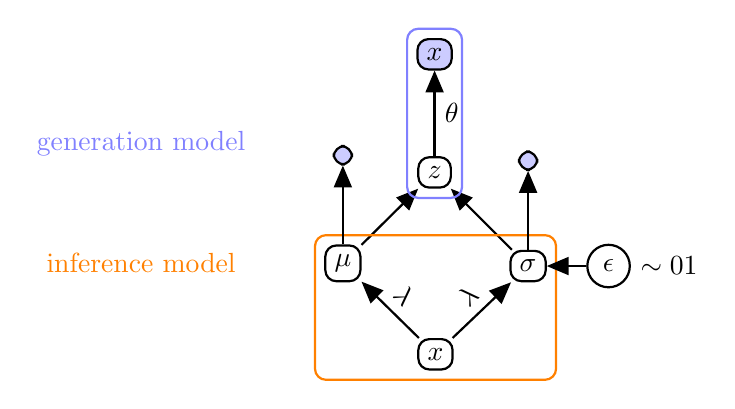
\begin{tikzpicture}[node distance=1cm]
\node[rectangle, draw, rounded corners, thick] (input) {$x$};
\node[rectangle, draw, rounded corners, thick, above left=of input] (mu) {$ \mu $};
\node[rectangle, draw, rounded corners, thick, above right=of input] (var) {$ \sigma $};
\node[rectangle, draw, rounded corners, thick, above right= of mu] (z) {$ z $};
\node[rectangle, fill=blue!20, thick, above of= z, rounded corners, draw, node distance=1.5cm] (output) {$ x $};

\draw[->, thick] (input) -- (mu) node[midway, above, rotate=315] {$ \lambda $};
\draw[->, thick] (input) -- (var) node[midway, above, rotate=45] {$ \lambda $};
\draw[->, thick] (mu) edge (z);
\draw[->, thick] (var) edge (z);
\draw[->, thick] (z) -- (output) node[midway, right] {$ \theta $};

\pause
\node[draw=orange, thick, rectangle, fit= (input) (mu) (var), rounded corners] {};
\node[left= of mu] (inference) {\textcolor{orange}{inference model}};

\pause
\node[draw=blue!50, thick, rectangle, fit= (z) (output), rounded corners] {};
\node[above= of inference] (generation) {\textcolor{blue!50}{generation model}};

\pause
\node[circle, draw, thick ,right =of var, xshift=-.5cm] (epsilon) {$ \epsilon $};
\node[right = of epsilon, xshift=-1cm] (stdNormal) {$ \sim \NDist{0}{1} $};
\draw[->, thick] (epsilon) edge (var);

\pause
\node[above= of mu, rectangle, fill=blue!20, thick, rounded corners, draw,] (KLmu) {$ \KullbackLeibler $};
\draw[->, thick] (mu) edge (KLmu);
\node[above= of var, rectangle, fill=blue!20, thick, rounded corners, draw,] (KLvar) {$ \KullbackLeibler $};
\draw[->, thick] (var) edge (KLvar);
\end{tikzpicture}
\end{figure}
\end{frame}


\begin{frame}{Example: Unigram Document Model}


\begin{columns}
	\begin{column}{0.2\textwidth}
	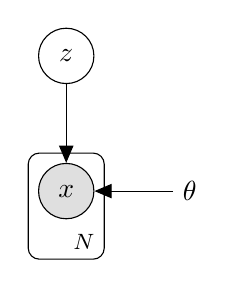
\begin{tikzpicture}
    % Define nodes
    \node[latent]		(z)		{$ z $};
    \node[obs, below = of z]		(x)		{$ x $};
    \node[right = of x]		(theta)		{$ \theta $};
    
    % Connect nodes
    \edge{z,theta}{x};
    
    % add plates
    \plate {x-sentence} {(x)} {$ N $};
   
    %\node[right = of z]		(lambda)		{$ \lambda $};   
    %\edge[dashed, bend right]{x}{z};
    %\edge{lambda}{z};
    \end{tikzpicture}
    \end{column}
    \begin{column}{0.75\textwidth}
    	Generative story 
    	\begin{itemize}
			\item Draw a document embedding $Z \sim \mathcal N(0, I)$
			\item Draw $N$ words\\
			$X_i|z \sim \Cat(f(z, \theta))$
		\end{itemize}
    \end{column}
    \end{columns}
    \pause
    
    ~
    
    Designing $f(z, \theta)$    \pause
    \begin{equation*}
	\begin{aligned}						
		h &= \relu(W_1z+b_1) \\ \pause
		f(z, \theta) &= \alert{\softmax}(W_2h + b_2) \\		\pause
		\theta &= \{W_1, b_1, W_2, b_2\}
	\end{aligned}
	\end{equation*}
	
	\pnote{Q: Why do we need a softmax?}

\end{frame}

\begin{frame}{Example: Unigram Document Model}


\begin{columns}
	\begin{column}{0.2\textwidth}
	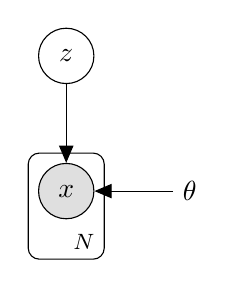
\begin{tikzpicture}
    % Define nodes
    \node[latent]		(z)		{$ z $};
    \node[obs, below = of z]		(x)		{$ x $};
    \node[right = of x]		(theta)		{$ \theta $};
    
    % Connect nodes
    \edge{z,theta}{x};
    
    % add plates
    \plate {x-sentence} {(x)} {$ N $};
   
    %\node[right = of z]		(lambda)		{$ \lambda $};   
    %\edge[dashed, bend right]{x}{z};
    %\edge{lambda}{z};
    \end{tikzpicture}
    \end{column}
    \begin{column}{0.75\textwidth}
    	Generative story 
    	\begin{itemize}
			\item Draw a document embedding $Z \sim \mathcal N(0, I)$
			\item Draw $N$ words\\
			$X_i|z \sim \Cat(f(z, \theta))$
		\end{itemize}
    \end{column}
    \end{columns}
    
    
    ~
    
	Likelihood \pause
	\begin{small}
    \begin{equation*}
	\begin{aligned}						
		p(x_1^N|z, \theta) &= \prod_{i=1}^N p(x_i|z, \theta) \pause = \prod_{i=1}^N \Cat(x_i|\underbrace{f(z, \theta)}_{=\psi}) \\ \pause
		&= \prod_{i=1}^N \psi_{x_i}
	\end{aligned}
	\end{equation*}
	\end{small}

\end{frame}


\begin{frame}{Example: Unigram Document Model}


\begin{columns}
	\begin{column}{0.2\textwidth}
	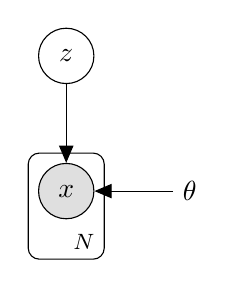
\begin{tikzpicture}
    % Define nodes
    \node[latent]		(z)		{$ z $};
    \node[obs, below = of z]		(x)		{$ x $};
    \node[right = of x]		(theta)		{$ \theta $};
    
    % Connect nodes
    \edge{z,theta}{x};
    
    % add plates
    \plate {x-sentence} {(x)} {$ N $};
   
    %\node[right = of z]		(lambda)		{$ \lambda $};   
    %\edge[dashed, bend right]{x}{z};
    %\edge{lambda}{z};
    \end{tikzpicture}
    \end{column}
    \begin{column}{0.75\textwidth}
    	Generative story 
    	\begin{itemize}
			\item Draw a document embedding $Z \sim \mathcal N(0, I)$
			\item Draw $N$ words\\
			$X_i|z \sim \Cat(f(z, \theta))$
		\end{itemize}
    \end{column}
    \end{columns}
    
    
    ~
    
	Marginal \pause
	\begin{small}
    \begin{equation*}
	\begin{aligned}						
		p(x_1^N|\theta) &= \int p(z) \prod_{i=1}^N p(x_i|z, \theta) \dd{z} \pause \\
		&= \alert{\int \mathcal N(z|0, I)} \prod_{i=1}^N \Cat(x_i|\alert{f(z, \theta)}) \alert{\dd{z}}
	\end{aligned}
	\end{equation*}
	\end{small}

\end{frame}

\begin{frame}{Example: Unigram Document Model}


\begin{columns}
	\begin{column}{0.75\textwidth}  
   		\textcolor{blue}{Inference model}
		\begin{itemize}
			\item $Z|x_1^N \sim \mathcal N(\mu(x_1^N, \lambda), \sigma(x_1^n, \lambda)^2)$
		\end{itemize}
    \end{column}
	\begin{column}{0.2\textwidth}
	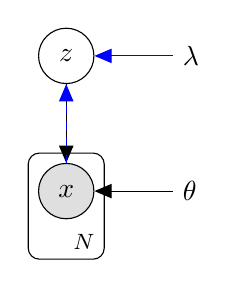
\begin{tikzpicture}
    % Define nodes
    \node[latent]		(z)		{$ z $};
    \node[obs, below = of z]		(x)		{$ x $};
    \node[right = of x]		(theta)		{$ \theta $};
    
    % Connect nodes
    \edge{z,theta}{x};
    
    % add plates
    \plate {x-sentence} {(x)} {$ N $};
   
    \node[right = of z]		(lambda)		{$ \lambda $};   
    \edge[dashed, blue, bend right]{x}{z};
    \edge[blue]{lambda}{z};
    \end{tikzpicture}
    \end{column}    
    \end{columns}
    \pause
    
    Designing the \emph{inference network}\pause
    \vspace{-10pt}
    \begin{columns}
    \begin{column}{0.35\textwidth}
    \begin{equation*}
	\begin{aligned}		
		s &= \sum_{i=1}^N E_{x_i} \pause \\
		h &= \relu(M_1s+c_1)  \pause 		
	\end{aligned}
	\end{equation*}
	\end{column}
	\begin{column}{0.6\textwidth}
	\begin{equation*}
	\begin{aligned}		
		\mu(x_1^N, \lambda) &= M_2h + c_2  \pause \\
		\sigma(x_1^N, \lambda) &= \alert{\softplus}(M_3h + c_3)  \pause \\
		\lambda &= \{E, M_1^3, c_1^3\}
	\end{aligned}
	\end{equation*}
	\end{column}
	\end{columns}
	
	\pnote{Q: Why do we need softplus?}

\end{frame}


\begin{frame}{Example: Unigram Document Model}

\begin{columns}
	\begin{column}{0.75\textwidth}  

		Generative Model
		\begin{itemize}
			\item Prior: $Z \sim \mathcal N(0, I)$
			\item Likelihood: $X_i|z \sim \Cat(f(z, \theta))$
		\end{itemize}
   		Inference Model
		\begin{itemize}
			\item $Z|x_1^N \sim \mathcal N(\mu(x_1^N, \lambda), \sigma(x_1^n, \lambda)^2)$
		\end{itemize}
    \end{column}
	\begin{column}{0.2\textwidth}
	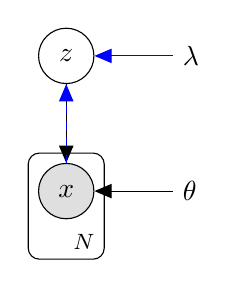
\begin{tikzpicture}
    % Define nodes
    \node[latent]		(z)		{$ z $};
    \node[obs, below = of z]		(x)		{$ x $};
    \node[right = of x]		(theta)		{$ \theta $};
    
    % Connect nodes
    \edge{z,theta}{x};
    
    % add plates
    \plate {x-sentence} {(x)} {$ N $};
   
    \node[right = of z]		(lambda)		{$ \lambda $};   
    \edge[dashed, blue, bend right]{x}{z};
    \edge[blue]{lambda}{z};
    \end{tikzpicture}
    \end{column}    
    \end{columns}
    \pause
    
    \vspace{10pt}
    
    \alert{ELBO}
    \vspace{-10pt}
	\begin{equation*}
	\begin{aligned}		
		\log p(x_1^N|\theta) &\ge \mathbb E_{\frac{z - u}{s} \sim \mathcal N(0, I)}\left[ \textstyle\sum_{i=1}^N \log \psi_{x_i}\right] \\
		&- \KL{\mathcal N(z|u, s^2)}{\mathcal N(z|0, I)}
	\end{aligned}
	\end{equation*}
	\textcolor{gray}{{\small where $u = \mu(x_1^N, \lambda)$, $s = \sigma(x_1^N, \lambda)$, and $\psi = f(z, \theta)$ }}

\end{frame}

\begin{frame}{Aside}
If your likelihood model is able to express dependencies between the output variables (e.g. an RNN), the model may simply ignore the latent code.
In that case one often scales the KL term. The scale factor is increased gradually.
\begin{equation*}
\E[q(z|x,\lambda)]{\log p(x|z,\theta)} - \beta \KL{q(z|x,\lambda)}{p(z)}
\end{equation*}
where $ \beta \rightarrow 1 $.
\end{frame}

\begin{frame}{Variational Autoencoder}
\textbf{Advantages}
\begin{itemize}
\item Backprop training
\item Easy to implement
\item Posterior inference possible
\item One objective for both NNs
\item Amortised inference
\end{itemize}
\pause
\textbf{Drawbacks}
\begin{itemize}
\item Discrete latent variables are difficult
\item Optimisation may be difficult with several latent variables
\end{itemize}
\end{frame}


\begin{frame}{What about amortised inference?}
\textcolor{blue}{Joint distribution:} latent variables are marginally independent a priori\\
$$\text{for example, }K=3, N=4$$
\begin{figure}
\center
\begin{tikzpicture}
\foreach \x in {1,...,4} {
  \pgfmathtruncatemacro{\y}{\x-1}
  \ifthenelse{\x=1}{\node[obs] (x\x) {$ x_{\x} $}}{\node[obs, right= of x\y] (x\x) {$ x_{\x} $}};
}
\foreach \z in {1,2,3} {
  \node[latent, above right = of x\z] (z\z) {$ z_{\z} $};
  \only<1>{\edge[blue]{z\z}{x1,x2,x3,x4};}
}
\foreach \z in {1,2,3} {
  \only<2>{\edge[red]{x1,x2,x3,x4}{z\z};}
}
\uncover<2->{
\edge[-,red]{z1}{z2};
\edge[-,red,bend left]{z1}{z3};
\edge[-,red]{z2}{z3};
}
\end{tikzpicture}
\end{figure}

~

\uncover<2>{\alert{Posterior: } latent variables are marginally dependent given observations}

%At inference time the latent variables are marginally dependent. For our variational distribution
%we are going to assume that they are not (recall: mean field assumption).
\end{frame}



\begin{frame}{Mean field assumption}

We have $K$ latent variables\\
\begin{itemize}
	\item assume the posterior factorises as $K$ independent terms
\end{itemize}


\begin{equation*}
q(z_1, \ldots, z_K) = \underbrace{\prod_{j=1}^K q_{\alert{\lambda_j}}(z_j)}_{\text{mean field}}
\end{equation*} \pause

with independent sets of parameters $\lambda_j = \{\mu_j, \sigma_j\}$
$$Z_j \sim \mathcal N(\mu_j, \sigma_j^2)$$

\end{frame}

\begin{frame}{Mean field: example}
\begin{figure}
\center
\begin{tikzpicture}
\foreach \x in {1,...,4} {
\pgfmathtruncatemacro{\y}{\x-1}
\ifthenelse{\x=1}{\node[obs] (x\x) {$ x_{\x} $}}{\node[obs, right= of x\y] (x\x) {$ x_{\x} $}};
}
\foreach \z in {1,2,3} {
  \node[latent, above right = of x\z] (z\z) {$ z_{\z} $};
  \edge[color=red]{x1,x2,x3,x4}{z\z};
  \node[above = of z\z] (lambda\z) {$ \lambda_{\z} $};
  \edge[color=red]{lambda\z}{z\z};
}
\end{tikzpicture}
\end{figure}

\end{frame}


\begin{frame}{Amortised variational inference}

Amortise the cost of inference using NNs
\begin{equation*}
q(z_1, \ldots, z_K|x) = \prod_{j=1}^K q_{\alert{\lambda}}(z_j|x)
\end{equation*} \pause
~ still mean field
$$Z_j|x \sim \mathcal N(\mu_j, \sigma_j^2)$$\\  \pause
~ but with a shared set of parameters
\begin{itemize}
	\item where $\mu_1^K, \sigma_1^K = g_{\alert{\lambda}}(x)$ 
\end{itemize}

\end{frame}


\begin{frame}{Amortised VI: example}
\begin{figure}
\center
\begin{tikzpicture}
\foreach \x in {1,...,4} {
\pgfmathtruncatemacro{\y}{\x-1}
\ifthenelse{\x=1}{\node[obs] (x\x) {$ x_{\x} $}}{\node[obs, right= of x\y] (x\x) {$ x_{\x} $}};
}
\foreach \z in {1,2,3} {
  \node[latent, above right = of x\z] (z\z) {$ z_{\z} $};
  \edge[color=red]{x1,x2,x3,x4}{z\z};
}
\node[above = of z2] (lambda) {$ \lambda $};
\foreach \z in {1,2,3} {
  \edge[color=red]{lambda}{z\z};
}
\end{tikzpicture}
\end{figure}

\end{frame}

\begin{frame}[plain]{Overview}

	\begin{minipage}[b][.35\textheight][t]{.47\textwidth}
	Joint\,distribution
	
	\vspace{10pt}
	
	\scalebox{0.9}{
	\begin{tikzpicture}
	\foreach \x in {1,...,4} {
	  \pgfmathtruncatemacro{\y}{\x-1}
	  \ifthenelse{\x=1}{\node[obs] (x\x) {$ x_{\x} $}}{\node[obs, right= of x\y] (x\x) {$ x_{\x} $}};
	}
	\foreach \z in {1,2,3} {
	  \node[latent, above right = of x\z] (z\z) {$ z_{\z} $};
	  \edge[blue]{z\z}{x1,x2,x3,x4};
	}
	\end{tikzpicture}}
	\end{minipage}\hfill%
    \begin{minipage}[b][.35\textheight][t]{.47\textwidth}
    Posterior
    \scalebox{0.9}{
    \begin{tikzpicture}
	\foreach \x in {1,...,4} {
	  \pgfmathtruncatemacro{\y}{\x-1}
	  \ifthenelse{\x=1}{\node[obs] (x\x) {$ x_{\x} $}}{\node[obs, right= of x\y] (x\x) {$ x_{\x} $}};
	}
	\foreach \z in {1,2,3} {
	  \node[latent, above right = of x\z] (z\z) {$ z_{\z} $};
	  \edge[red]{x1,x2,x3,x4}{z\z};
	}
	\edge[-,red]{z1}{z2};
	\edge[-,red,bend left]{z1}{z3};
	\edge[-,red]{z2}{z3};
	\end{tikzpicture}
    }
    \end{minipage}\\[0.5em]
    \begin{minipage}[b][.35\textheight][t]{.47\textwidth}
    Mean\,field
    \scalebox{0.9}{
	\begin{tikzpicture}
	\foreach \x in {1,...,4} {
	\pgfmathtruncatemacro{\y}{\x-1}
	\ifthenelse{\x=1}{\node[obs] (x\x) {$ x_{\x} $}}{\node[obs, right= of x\y] (x\x) {$ x_{\x} $}};
	}
	\foreach \z in {1,2,3} {
	  \node[latent, above right = of x\z] (z\z) {$ z_{\z} $};
	  \edge[color=red]{x1,x2,x3,x4}{z\z};
	  \node[above = of z\z] (lambda\z) {$ \lambda_{\z} $};
	  \edge[color=red]{lambda\z}{z\z};
	}
	\end{tikzpicture}}
    \end{minipage}\hfill
    \begin{minipage}[b][.35\textheight][t]{.47\textwidth}
    Amortised\,VI
    \scalebox{0.9}{
	\begin{tikzpicture}
	\foreach \x in {1,...,4} {
	\pgfmathtruncatemacro{\y}{\x-1}
	\ifthenelse{\x=1}{\node[obs] (x\x) {$ x_{\x} $}}{\node[obs, right= of x\y] (x\x) {$ x_{\x} $}};
	}
	\foreach \z in {1,2,3} {
	  \node[latent, above right = of x\z] (z\z) {$ z_{\z} $};
	  \edge[color=red]{x1,x2,x3,x4}{z\z};
	}
	\node[above = of z2] (lambda) {$ \lambda $};
	\foreach \z in {1,2,3} {
	  \edge[color=red]{lambda}{z\z};
	}
	\end{tikzpicture}}
    \end{minipage}%
\end{frame}




\begin{frame}{Summary}
\begin{itemize}
%\item When $ |\mathcal{X}| $ and $ |\mathcal{Z}| $ are not too large, we can do EM with features
%\item Otherwise use VI with simple approximation
\item Wake-Sleep: train inference and generation networks with separate objectives
\item VAE: train both networks with same objective
\item Reparametrisation
\begin{itemize}
\item  Transform parameter-free variable $ \epsilon $ into latent value $ z $
\item Update parameters with stochastic gradient estimates
\end{itemize}
\end{itemize}
\end{frame}

\begin{frame}[allowframebreaks]{Literature}
\nocite{KingmaWelling:2013}
\nocite{HintonEtAl:1995}
\nocite{RezendeEtAl:2014}
\nocite{TitsiasLazarogredilla:2014}
%\nocite{BergkirkpatrickEtAl:2010}
\nocite{KucukelbirEtAl:2017}

\bibliographystyle{plainnat}
\bibliography{../../VI}
\end{frame}

\end{document}